\documentclass[a4paper,10pt]{article}
\usepackage[utf8]{inputenc}
\usepackage{lmodern}
\usepackage[T1]{fontenc}
\usepackage[italian]{babel}

\usepackage{amsmath}
\usepackage{amsfonts}
\usepackage{amssymb}

\usepackage{graphicx}
\usepackage[dvipsnames]{xcolor}  %colori

\usepackage{pgf}
\usepackage{tikz}
\usetikzlibrary{arrows,shapes,snakes,automata,backgrounds,petri}	% Finite States Machine

\usepackage[left=2cm,right=2cm,top=2cm,bottom=2cm]{geometry}
\geometry{a4paper}
\setlength\marginparwidth{40pt}
\setlength\marginparsep{1pt}

\usepackage{verbatim}
\usepackage{lipsum}

\usepackage{booktabs}
\usepackage{subfig}
\usepackage{float}
\usepackage{wrapfig}

\usepackage[colorlinks=true, linkcolor=black, urlcolor=blue, citecolor=darkgray, filecolor=darkgray]{hyperref}   %per gli hyperlink
\usepackage[italian, sort, noabbrev, capitalise]{cleveref}
\usepackage[bottom]{footmisc}

\usepackage[cdot, thickqspace, squaren]{SIunits}
% macro
\def\code#1{\texttt{#1}}

\title{Esercitazione 15: Misura della costante di Boltzmann attraverso misure di rumore}
\author{Gruppo BL \\ Candido Alessandro, Luzio Andrea, Mazziotti Fabrizio}

\begin{document}

\maketitle

\section{Scopo e Strumentazione}
In questa esercitazione si vuole effettuare una misura della costante di Boltzmann attraverso la
misura del rumore termico in una serie di resistenze con valori diversi.

\noindent La strumentazione è quella solitamente presente sul banco di lavoro, e inoltre si è usato:
\begin{itemize}
	\item INA114: Precision instrumentation amplifier;
	\item AD708: ultra low offset dual op-amp (2 integrati);
	\item AD736: true rms-to-dc converter.
\end{itemize}

\subsubsection*{Schema complessivo}

Lo schema a blocchi del circuito è riportato in \cref{fig:blocks}.

\begin{figure}[H]
	\centering
	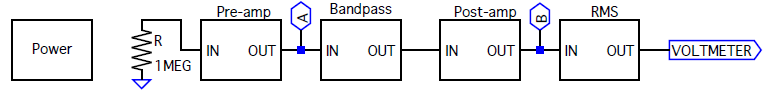
\includegraphics[width=\textwidth]{../grafici/Blocks.png}
	\vspace*{10pt}
	\caption{Schema a blocchi del circuito complessivo.}
	\label{fig:blocks}
\end{figure}

\begin{wrapfigure}{L}{0.35\textwidth}
	\vspace{-10pt}
	\centering
	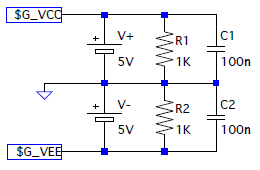
\includegraphics[width=0.35\textwidth]{../grafici/Filter.png}
	\vspace{-6pt}
	\caption{Schema di filtraggio per le alimentazioni.}
	\label{fig:powamp}
	\vspace{-12pt}
\end{wrapfigure}

\lipsum[1-2]

\pagebreak

\section{Implementazione dei blocchi di circuito}

\subsection{Pre-amplificatore}

\begin{wrapfigure}{L}{0.6\textwidth}
	\vspace{-10pt}
	\centering
	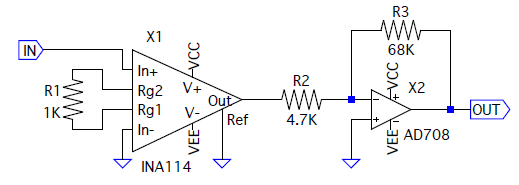
\includegraphics[width=0.6\textwidth]{../grafici/PreAmp.png}
	\vspace{-12pt}
	\caption{Schema del circuito: pre-amplificatore.}
	\label{fig:powamp}
	\vspace{-6pt}
\end{wrapfigure}

\lipsum[2-3]

\subsubsection*{Amplificazione e risposta in frequenza}

\lipsum[4]

\subsection{Filtro passabanda e post-amplificatore}

\begin{wrapfigure}{R}{0.5\textwidth}
	\vspace{-10pt}
	\centering
	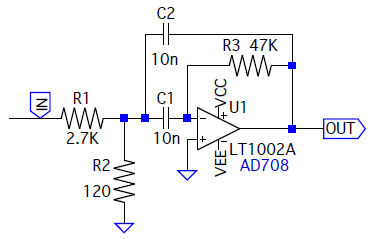
\includegraphics[width=0.5\textwidth]{../grafici/Bandpass.png}
	\vspace{-12pt}
	\caption{Schema del circuito: filtro passabanda.}
	\label{fig:powamp}
	\vspace{-6pt}
\end{wrapfigure}

\lipsum[4-5]

\begin{wrapfigure}{L}{0.6\textwidth}
	\vspace{-10pt}
	\centering
	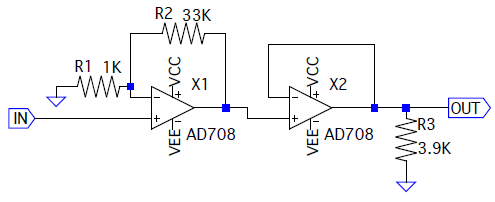
\includegraphics[width=0.6\textwidth]{../grafici/PostAmp.png}
	\vspace{-12pt}
	\caption{Schema del circuito: post-amplificatore.}
	\label{fig:powamp}
	\vspace{-6pt}
\end{wrapfigure}

\lipsum[6-7]

\subsubsection*{Amplificazione e risposta in frequenza}

\lipsum[4]

\begin{figure}[H]
	\centering
	\includegraphics[width=0.7\textwidth]{../grafici/passabanda.pdf}
	\vspace*{10pt}
	\caption{Amplificazione e risposta in frequenza degli stadi passabanda e post-amplificatore in serie.}
	\label{fig:blocks}
\end{figure}

\subsection{Convertitore RMS}

\begin{wrapfigure}{L}{0.4\textwidth}
	\vspace{-10pt}
	\centering
	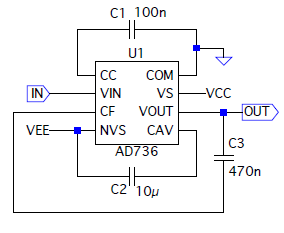
\includegraphics[width=0.4\textwidth]{../grafici/RMSconverter.png}
	\vspace{-12pt}
	\caption{Schema del circuito: convertitore RMS.}
	\label{fig:powamp}
	\vspace{-6pt}
\end{wrapfigure}

\lipsum[2-5]

\subsubsection*{Calibrazione}

\lipsum[4]

\begin{figure}[H]
	\centering
	\includegraphics[width=0.7\textwidth]{../grafici/calibrazione.pdf}
	\vspace*{10pt}
	\caption{Fit della calibrazione del convertitore RMS.}
	\label{fig:blocks}
\end{figure}

\section{Analisi complessiva} % questo nome si può anche cambiare, non è che mi piaccia un granché

\subsection{Stima diretta dell'amplificazione \\e risposta in frequenza del circuito complessivo}

\lipsum[8]

\subsection{Risultati finali}

\lipsum[9]

\end{document}